eKwip consists of several components that all work together to collect data about the position and motion of the knee and leg, store the data locally, send the data over a wireless network link to a server, and analyze the data in order to display an image of the knee and compute a KIRI score.

The process begins in the IMU sensors, which use accelerometers and gyroscopes to measure the absolute orientation, acceleration, and rate of change of acceleration. This data is passed to the microcontroller, which packetizes the data and send it to the wireless module, which transmits the data packets over the wireless network to the server.

The server receives the data packets and parses the data. It then computes the position and movement of the knee in order to display the image of the leg in the graphical user interface. Additionally, the server will compute the KIRI score for the individual and display that value.

Figure~\ref{fig:block_diagram} shows a block diagram modelling the eKwip system.

\begin{figure}[h]
  \begin{center}
    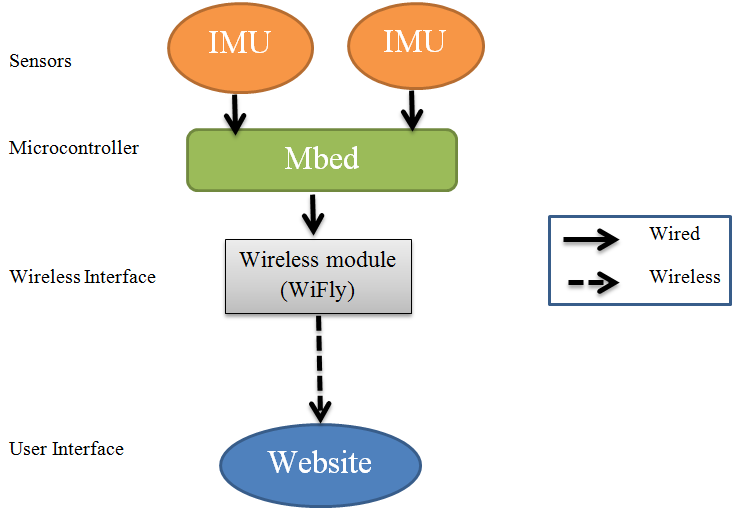
\includegraphics[width=3in]{images/block_diagram.PNG}
  \end{center}
  \caption{Block diagram of eKwip system}
  \label{fig:block_diagram}
\end{figure}